\documentclass{article}

\usepackage{amsmath}
\usepackage{amsfonts}
\usepackage{amssymb}
\usepackage{graphicx}
\usepackage{float}
\usepackage{hyperref}
\usepackage{subfig}
\usepackage[margin=0.75in]{geometry}
\graphicspath{{./assets/}}

\begin{document}

\section{Introduction}

    One time when I was binging YouTube, I stumbled upon a video by Grant Sanderson
    of 3Blue1Brown on Fourier series which featured many visualizations, prime of
    whose were drawings on a complex plain which were generated using Fourier
    series. Having done some reading on Fourier series as well as Fourier transform, 
    I decided that it would be a great idea to actually understand those concepts.
    Since for me the ultimate way of learning is solving problems and since I feel
    best at expressing ideas in code, I decided to set myself a challenge of 
    programming a program that will redraw my sketches with Fourier series.

\section{Overview of the program}

    The program has three main stages: 
    \begin{enumerate}
        \item taking input in the form of drawing from the user 
        \item processing the drawing using discrete Fourier transform (DFT)
        \item printing the drawing using discrete Fourier Series
    \end{enumerate}
    
    The output of the program is the following: (ADD IMAGES)



\section{What is Fourier series?}

    The purpose of Fourier series is to approximate any periodic function with
    a sum of sines and cosines. The formula is given by~\eqref{eq:fs_rbase}
    \begin{equation} \label{eq:fs_rbase}
        S_\infty(t) = a_0 + \sum_{n=1}^{\infty}a_ncos\frac{2\pi nt}{P} + b_n%
            sin\frac{2\pi nt}{P}
    \end{equation}
    From the formula we can observe two things, each sine and cosine in the sum
    has a weight assigned to it ($a_n$ and $b_n$) and that $n$ determines the 
    frequency of the sinusoids. We can demistify the idea behind Fourier series
    by deriving formulas for all coefficients.

\subsection{Deriving $a_0$}
    
    First coefficient we will find is $a_0$, which is the only coefficient that 
    stands on its own. It is added before the actual series in order to compensate
    for the original function not oscillating around $x$ axis on the plot. It 
    basically is a vertical translation. We can see it if we add any constant
    to $sin(x)$~\ref{fig:sine_translation}.
    \begin{figure}[H]
        \caption{red - $sin(x)$, blue - $3 + sin(x)$}
        \centering
        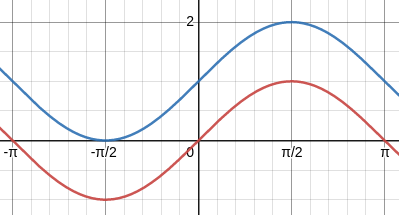
\includegraphics[width=0.5\linewidth]{translated_vanilla_sinewave}
        \label{fig:sine_translation}
    \end{figure}
    Now the problem to solve is what it the axis around which our sum of sines
    and cosines is to oscillate against. The solution to this problem is the average
    value of the original function over one period. The formula given for finding
    $a_0$ goes as follows~\eqref{eq:a0_formula}
    \begin{equation}\label{eq:a0_formula}
        a_0 = \frac{1}{P}\int_{\frac{P}{2}}^{\frac{-P}{2}}f(t)dt
    \end{equation}
    Now, how does an integral grant us mean value of a function? Well, definite
    integral gives us the area under the graph of function $f(t)$ from 
    $-\frac{1}{P}$ to $\frac{1}{P}$. If we have an area, we can express it with 
    any figure that has this area, since we want an offset from the $x$ axis, 
    we can draw a rectangle whose base has length of $P$. Sine we want to find
    out what the height of that rectangle is, we need to divide its area by its
    width, which is exactly what we are doing when dividing the integral by $P$.

\subsection{Finding $a_n$ and $b_n$}

    Weights $a_n$ and $b_n$ allow for the series to converge to desired function, 
    which is quite obvious from the fact that the series is infinite, which means
    that the values on their own would shoot up to infinity. Now, how are we to 
    find those weights to force the sinusoids to compliance? We can start with 
    equating some function $f(t)$ to a Fourier series~\eqref{eq:eq_fs_f(t)}
    \begin{equation} \label{eq:eq_fs_f(t)}
        f(t) = a_0 + \sum_{n=1}^{\infty}a_ncos\frac{2\pi nt}{P} + b_n%
            sin\frac{2\pi nt}{P}
    \end{equation}
    In order to find the coefficients, we can exploit the properties of definite
    integrals of sine and cosine. To do that, we will need to expand the whole 
    expression by either $cos\frac{2\pi nt}{P}$ when looking for $a_n$, or by 
    $sin\frac{2\pi nt}{P}$ if we are looking for $b_n$. Now we will go through 
    the whole process by looking for $a_n$. 


    The expanded equation we will use to find $a_n$ looks like this~\eqref{eq:fs_exp_cos}.
    \begin{equation}\label{eq:fs_exp_cos}
    \begin{split}
        \int_{-\frac{P}{2}}^{\frac{P}{2}}f(t)cos\frac{2\pi nt}{P}dt 
        & = \int_{-\frac{P}{2}}^{\frac{P}{2}}a_0cos\frac{2\pi nt}{P}dt+ 
        \int_{-\frac{P}{2}}^{\frac{P}{2}}a_1cos\frac{2\pi t}{P}cos\frac{2\pi nt}{P}dt +
        \int_{-\frac{P}{2}}^{\frac{P}{2}}b_1sin\frac{2\pi t}{P}cos\frac{2\pi nt}{P}dt \\
        & + \int_{-\frac{P}{2}}^{\frac{P}{2}}a_2cos\frac{4\pi t}{P}cos\frac{2\pi nt}{P}dt +
        \int_{-\frac{P}{2}}^{\frac{P}{2}}b_2sin\frac{4\pi t}{P}cos\frac{2\pi nt}{P}dt \\
        & \vdots \\
        & + \int_{-\frac{P}{2}}^{\frac{P}{2}}a_ncos^2(\frac{2\pi nt}{P})dt +
        \int_{-\frac{P}{2}}^{\frac{P}{2}}b_nsin\frac{2\pi nt}{P}cos\frac{2\pi nt}{P}dt 
    \end{split}
    \end{equation}
    From this rather long expansion we can distill and solve for five cases appearing
    on the right side of the equation:
    \begin{enumerate}
        \item \begin{equation*}
                \int_{-\frac{P}{2}}^{\frac{P}{2}}a_0cos\frac{2\pi nt}{P}dt
                = a_0 \cdot \left[\frac{P}{2\pi nt}sin\frac{2\pi nt}{P}\right]_{-\frac{P}{2}}^{\frac{P}{2}}
                = a_0 \cdot \frac{P}{2\pi nt}(sin(\pi n) - sin(-\pi n)) = 0
              \end{equation*}
        \item let $m \in Z \land m \neq n$
            \begin{equation*}
            \begin{split}
                \int_{-\frac{P}{2}}^{\frac{P}{2}}a_mcos\frac{2\pi mt}{P}cos\frac{2\pi nt}{P}dt 
                & = a_m \cdot \int_{-\frac{P}{2}}^{\frac{P}{2}}\frac{1}{2}\left(cos\frac{(m-n)2 \pi t}{P} + 
                cos\frac{(m+n)2 \pi t}{P}\right)dt \\
                & = a_m \cdot \left[\frac{P}{4\pi(m-n)}sin\frac{(m-n)2 \pi t}{P}
                + \frac{P}{4\pi(m+n)}sin\frac{(m+n)2 \pi t}{P}\right]_{-\frac{P}{2}}^{\frac{P}{2}} \\
                & = a_m \cdot (\frac{P}{4\pi(m-n)}sin((m-n)\pi) + \frac{P}{4\pi(m+n)}sin(-(m+n)\pi) = 0
            \end{split}
            \end{equation*}
        \item let $m \in Z$
            \begin{equation*}
            \begin{split}
                \int_{-\frac{P}{2}}^{\frac{P}{2}}b_msin\frac{2\pi mt}{P}cos\frac{2\pi nt}{P}dt 
                & = b_m \cdot \int_{-\frac{P}{2}}^{\frac{P}{2}}\frac{1}{2}\left(sin\frac{(m+n)2 \pi t}{P} + 
                sin\frac{(m+n)2 \pi t}{P}\right)dt \\
                & = b_m \cdot \left[\frac{-P}{4\pi(m+n)}cos\frac{(m+n)2 \pi t}{P}
                + \frac{-P}{4\pi(m+n)}cos\frac{(m+n)2 \pi t}{P}\right]_{-\frac{P}{2}}^{\frac{P}{2}} \\
                & = b_m \cdot (\frac{-P}{4\pi(m-n)}cos((m-n)\pi) + \frac{-P}{4\pi(n+m)}cos(-(m+n)\pi) = 0
            \end{split}
            \end{equation*}
        \item 
            \begin{equation*}
            \begin{split}
                \int_{-\frac{P}{2}}^{\frac{P}{2}}cos^2(\frac{2\pi nt}{P})dt
                & = \frac{1}{2}\int_{-\frac{P}{2}}^{\frac{P}{2}}1 + cos\frac{4\pi nt}{P}dt 
                = \frac{1}{2} \cdot \left[t + \frac{P}{4\pi nt}sin\frac{4\pi nt}{P}
                \right]_{-\frac{P}{2}}^{\frac{P}{2}} \\
                & = \frac{1}{2} \cdot \left(\frac{P}{2} + \frac{1}{2\pi n}sin(2\pi n)
                + \frac{P}{2} + \frac{1}{2\pi n}sin(-2\pi n)\right) = \frac{2}{P}
            \end{split}
            \end{equation*}
    \end{enumerate}

    We can see that the only term after expansion and integration that does not 
    amount to zero is $\int_{-\frac{P}{2}}^{\frac{P}{2}}cos^2(\frac{2\pi nt}{P})dt$,
    which means that our equation will simplify to the following form~\eqref{eq:fs_simp_cos}
    \begin{equation}\label{eq:fs_simp_cos}
        \int_{-\frac{P}{2}}^{\frac{P}{2}}f(t)cos\frac{2\pi nt}{P}dt = a_n\frac{P}{2}
    \end{equation}
    So in order to find $a_n$, we will get the following\eqref{eq:a_n}
    \begin{equation}\label{eq:a_n}
        a_n = \frac{2}{P}\int_{-\frac{P}{2}}^{\frac{P}{2}}f(t)cos\frac{2\pi nt}{P}dt
    \end{equation}
    Formula for $b_n$ is very similar~\eqref{eq:b_n} and stems from the same logic as one of 
    $a_n$, see Appendix A for calculations.
    \begin{equation}\label{eq:b_n}
        b_n = \frac{2}{P}\int_{-\frac{P}{2}}^{\frac{P}{2}}f(t)sin\frac{2\pi nt}{P}dt
    \end{equation}

\subsection{Approximating a step function}
    
    Before diving straight to other concepts and the drawings, let us 
    take a second and manually approximate a step function~\eqref{eq:step}.

    \begin{equation}\label{eq:step}
    \begin{split}
         &f(t) = 
        \begin{cases} 
            & -5 \text{ if } \frac{-P}{2} \leq t < 0 \\
            & 5 \text{ if }  0 \leq t \leq \frac{P}{2}
        \end{cases} \\
        & f(t) = f(t + P) 
    \end{split}
    \end{equation}


\end{document}
